\documentclass{beamer}

\usepackage[T1]{fontenc}
\usepackage[utf8]{inputenc}
\usepackage[slovene]{babel}
\usepackage{palatino}
\usefonttheme{serif}
\usepackage{amsmath,amssymb,amsfonts, mathtools}
\graphicspath{{./images/}}

\usetheme{CambridgeUS}
\usecolortheme{dolphin}
\setbeamertemplate{navigation symbols}{}

\linespread{1.2}

\newcommand{\N}{\mathbb{N}}
\newcommand{\Z}{\mathbb{Z}}
\newcommand{\Q}{\mathbb{Q}}
\newcommand{\R}{\mathbb{R}}
\newcommand{\C}{\mathbb{C}}

\theoremstyle{definition} % tekst napisan pokoncno
\newtheorem{definicija}{Definicija}[section]

\newcommand\Vtextvisiblespace[1][.3em]{%
\mbox{\kern.06em\vrule height.3ex}%
\vbox{\hrule width#1}%
\hbox{\vrule height.3ex}}

\title[Gramatike za kodiranje podatkov]{Kontekstno-neodvisne gramatike za kodiranje in stiskanje podatkov}
\author{Janez Podlogar}
\institute[UL-FMF]{Univerza v Ljubljani, Fakulteta za matematiko in fiziko}
\date[November 2022]{21. 11. 2022}

\begin{document}

\begin{frame}
    \titlepage
\end{frame}

\section{Kodiranje podatkov}

\begin{frame}{Kodiranje in kod}

\begin{columns}[c]
    \begin{column}{.5\textwidth}
        \begin{figure}
            \centering
            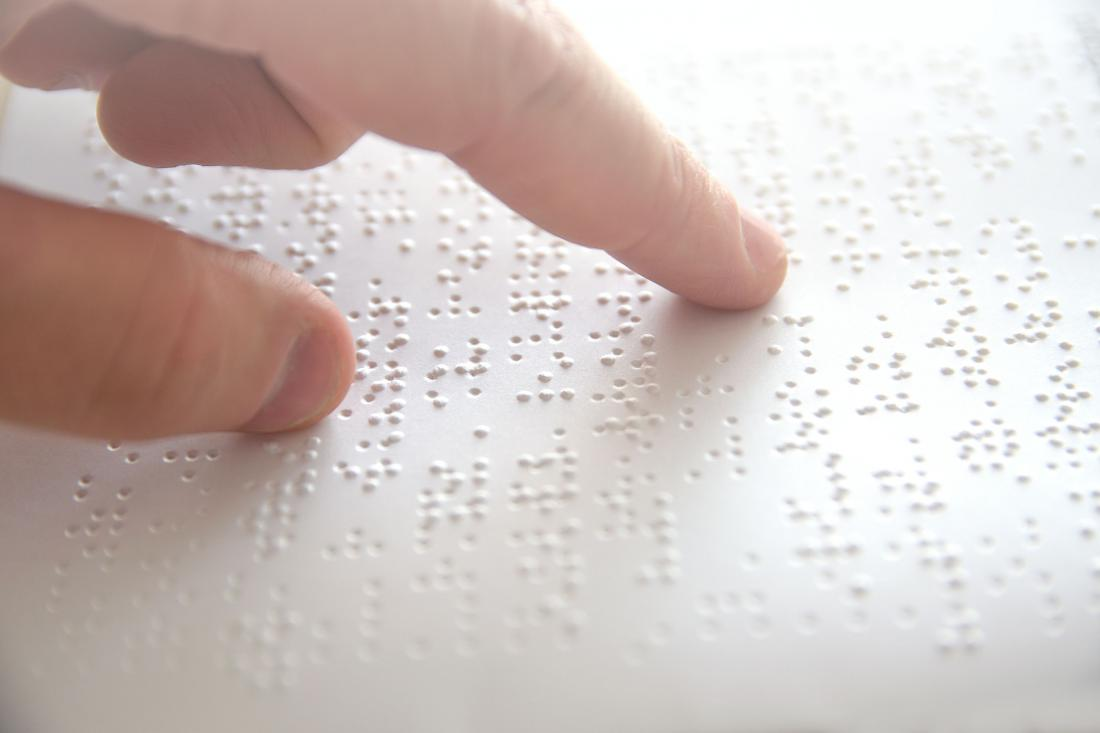
\includegraphics[width=0.8\textwidth]{Braillova_pisava.jpg}
            \caption{Telegrafska tipka in zvočnik}
        \end{figure}
    \end{column}

    \begin{column}{.5\textwidth}
        \begin{figure}
            \centering
            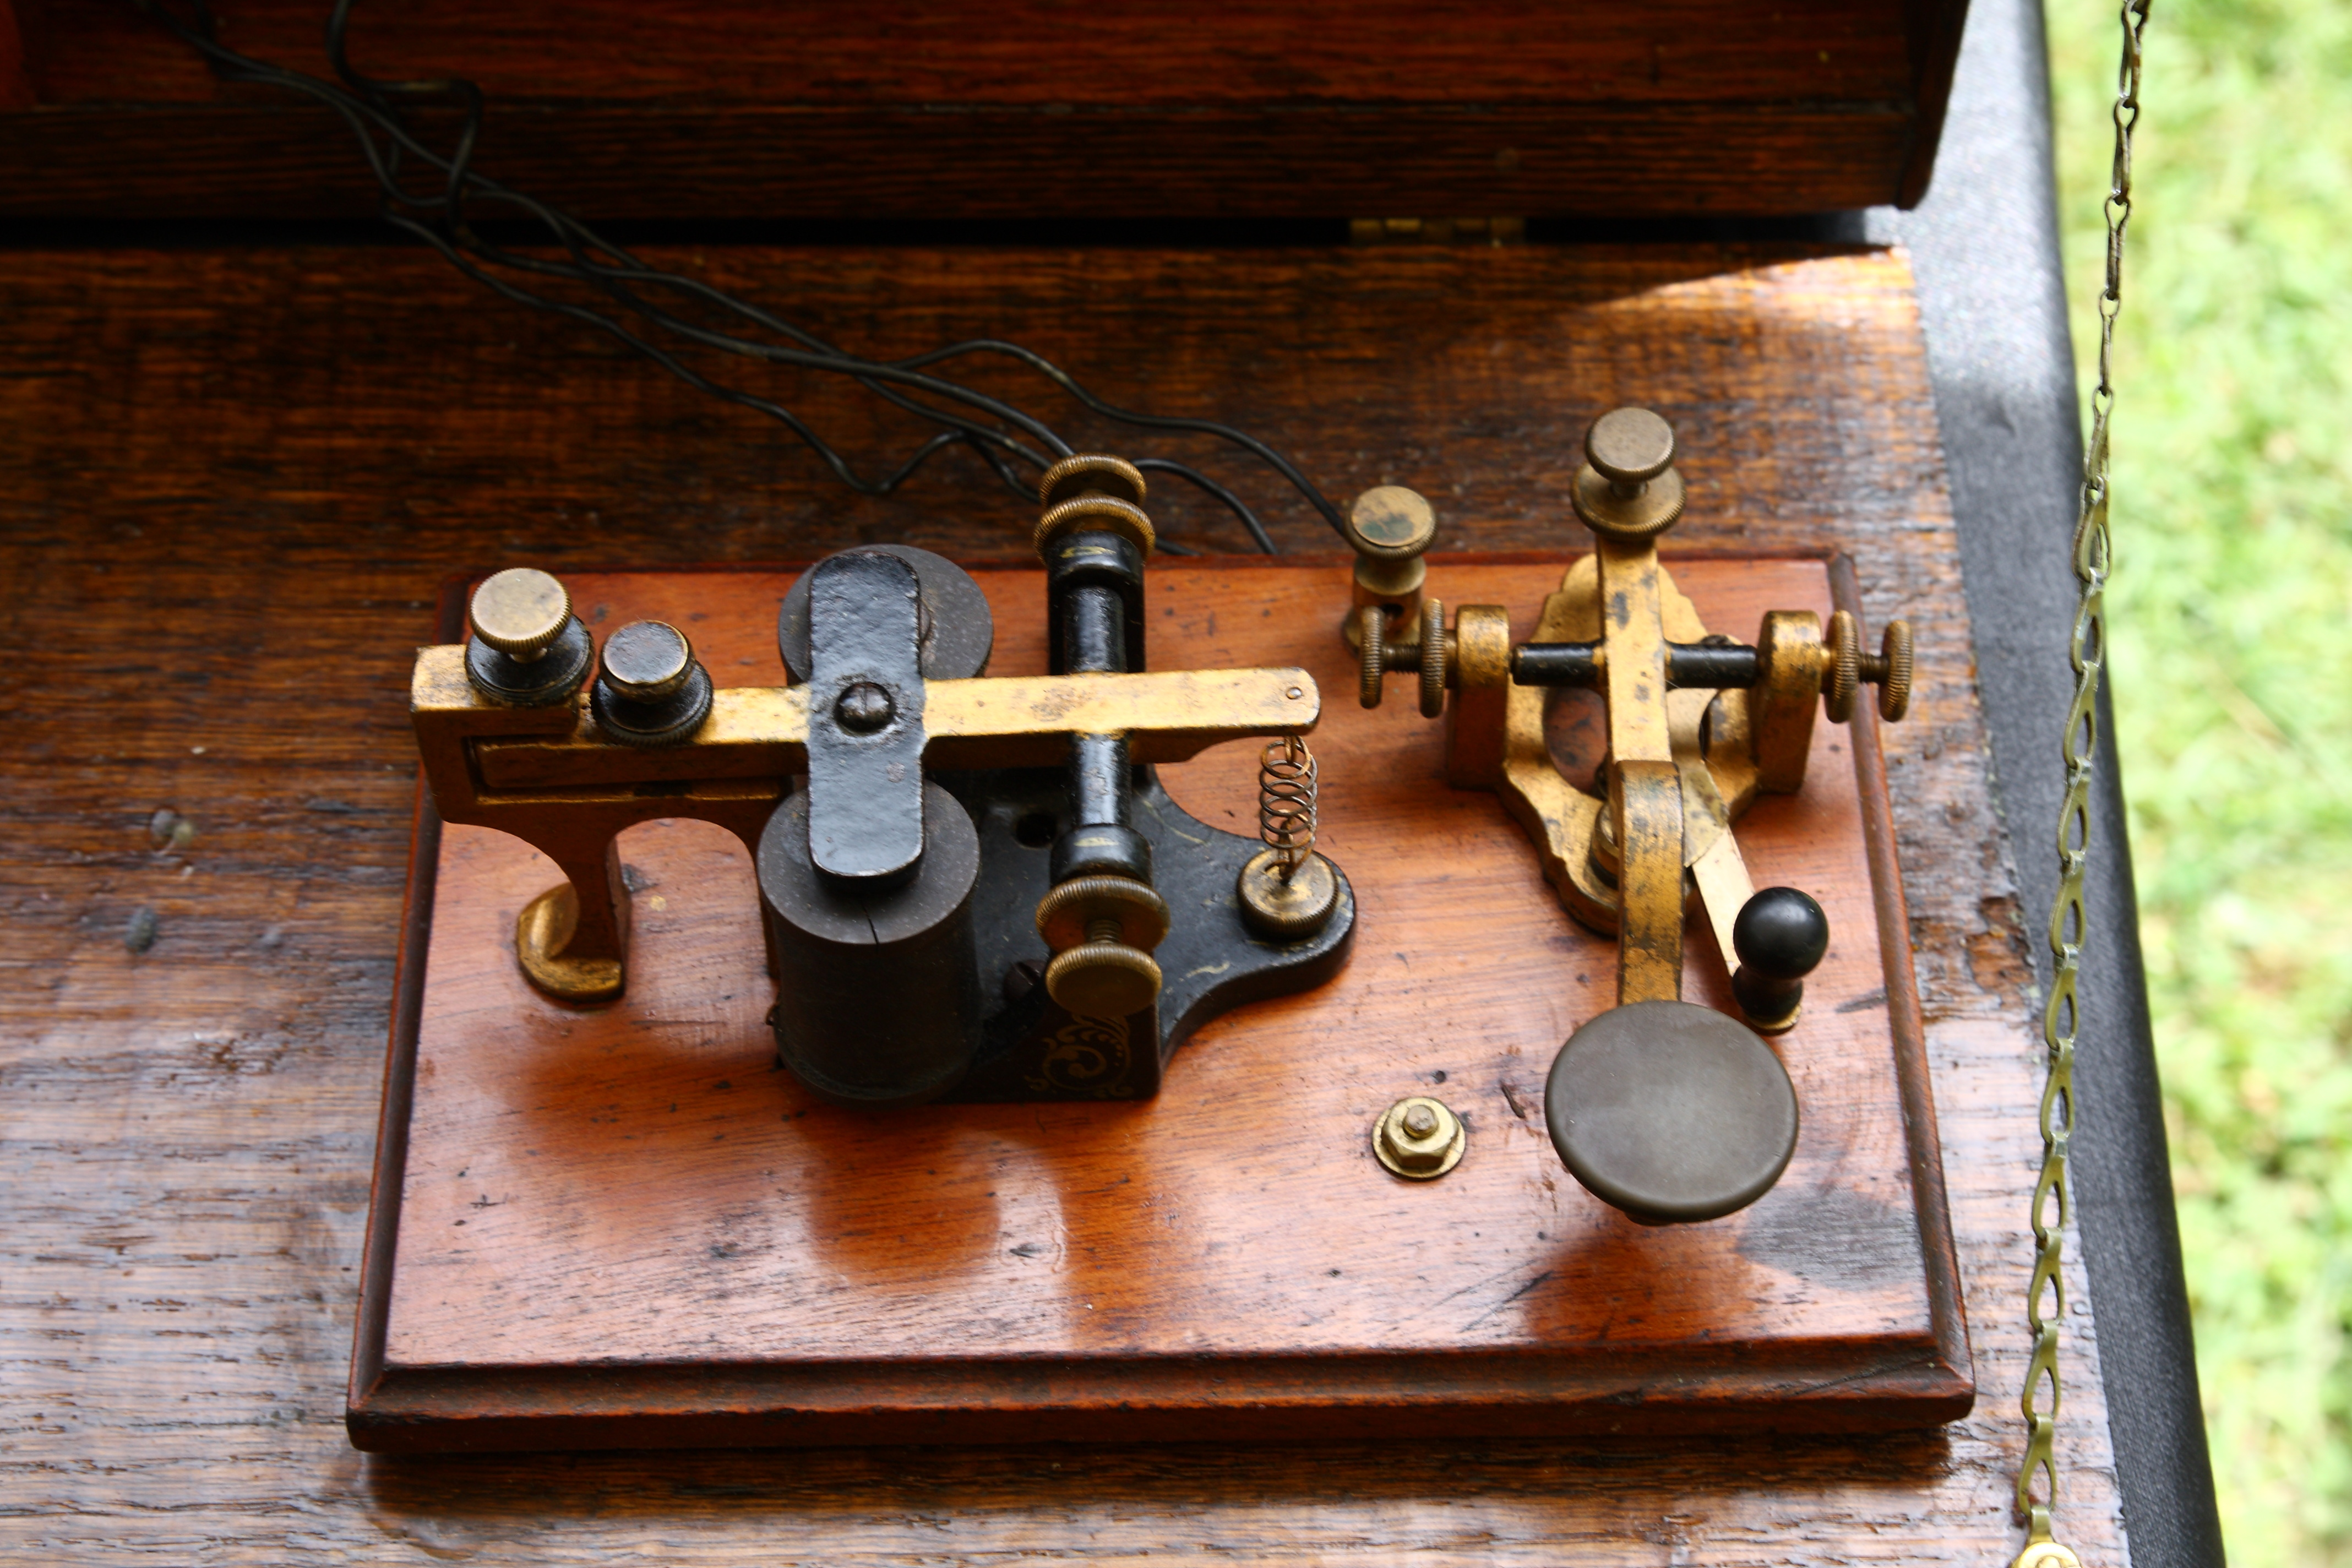
\includegraphics[width=0.8\textwidth]{Key_Sounder.jpg}
            \caption{Braillova pisava}
        \end{figure}
    \end{column}
\end{columns}

\end{frame}

\begin{frame}{Kodiranje in kod}
    \begin{itemize}
        \item<1-> Spreminjanje zapisa sporočila imenujemo \textit{kodiranje}
        \item<2-> Sistem pravil po katerem se kodiranje opravi imenujemo \textit{kod}
    \end{itemize}
\end{frame}

\begin{frame}{Morsejeva abeceda}
    \textit{Morsejeva abeceda} je kodiranje črk, števil in ločil s pomočjo zaporedja signalov:
    \begin{itemize}
        \item<2-> Dolžina kratkega signala je ena enota
        \item<3-> Dolgi signal je trikrat daljši od kratkega signala
        \item<4-> Razmik med signali znotraj črke je tišina dolžine kratkega signala
        \item<5-> Razmik med črkami je tišina dolga tri kratke signale oz. en dolgi signal
        \item<6-> Presledek med besedami je tišina dolga sedmih kratkih signalov
    \end{itemize}
\end{frame}

\begin{frame}{Abeceda in nizi na abecedi}
    \begin{definicija}
        \begin{itemize}
            \item \textit{Abeceda} je končna neprazna množica $ \Sigma $
            \item \textit{Množica vseh končnih nizov abecede} $ \Sigma $ označimo z $ \Sigma^* $
        \end{itemize}
    \end{definicija}    
    \begin{exampleblock}{Primer nizov abecede}<2->
    Naj bo $ \Sigma = \{ a,b,c \} $ abeceda, potem sta niza
    \[ 
        ab \in \Sigma^* , \quad cababcccababcccab \in \Sigma^*
    \]
    \end{exampleblock}
\end{frame}

\begin{frame}{Kodiranje in dekodiranje}
    \begin{definicija}
        \begin{itemize}
            \item \textit{Kodiranje nizov abecede} $ \Sigma $ je injektivna funkcija $ \kappa \colon \Sigma^* 
            \to \Sigma_c^* $
            \item<2-> \textit{Dokodiranje kodiranja} $ \kappa $ je funkcija 
            $ \delta \colon C \subseteq \Sigma^*_c \to \Sigma^* $, da velja
            \[
                \forall w \in \Sigma^* \colon \delta(\kappa(w)) = w
            \]
        \end{itemize}
    \end{definicija}
\end{frame}

\begin{frame}{Morsejeva abeceda}
    \begin{block}{Morsov kod}
        \begin{itemize}
            \item<2->  $ \Sigma = \{ \text{A},  \text{B}, \ldots, \text{Z} \} \cup \{ 0, 1, \ldots, 9 \}
            \cup \{ \Vtextvisiblespace[5pt] \} $
            \item<3-> $ \Sigma_c = \{ \cdot ,-, \Box \} $
            \item<4-> $ \kappa_s \colon \Sigma \to \Sigma_c^* $ \\ \phantom{}
        \end{itemize}
    \end{block}
\end{frame}

\begin{frame}
    \begin{block}{Kodna funkcija črk $ \kappa_s $}
        \begin{itemize}
            \item Vrednosti funkcije so določene s tabelo
            \begin{figure}[h]
                \centering
                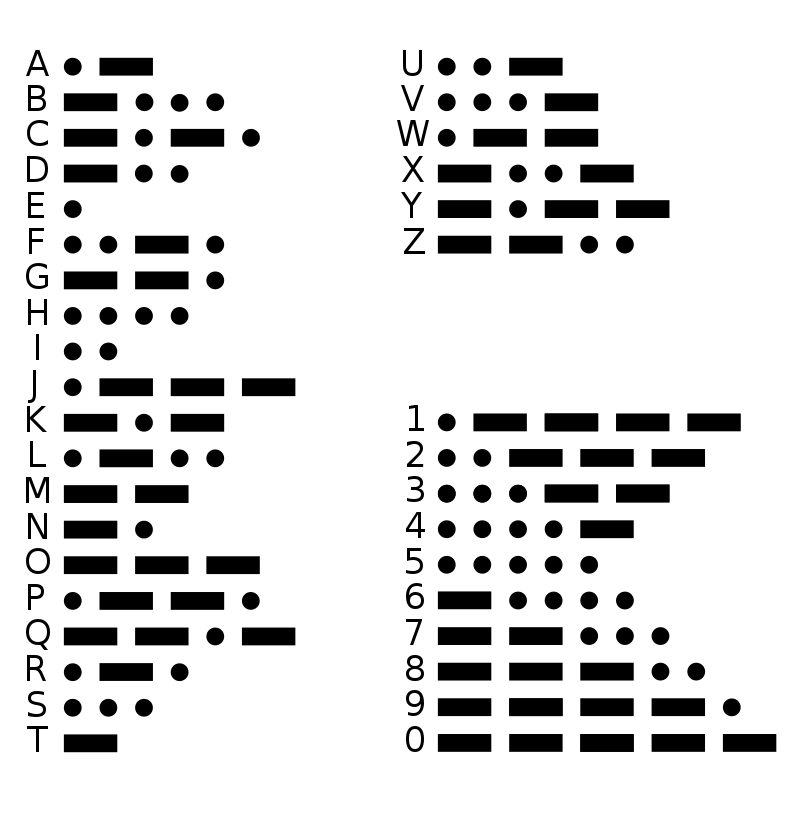
\includegraphics[width=3.5cm]{International_Morse_Code.svg.png}
            \end{figure}
            \item Dodatno $ \kappa_s(\Vtextvisiblespace[5pt]) = \Box\Box\Box $
        \end{itemize}
    \end{block}
\end{frame}

\begin{frame}{Morsejeva abeceda}
    \begin{block}{Morsov kod}
        \begin{itemize}
            \item  $ \Sigma = \{ \text{A},  \text{B}, \ldots, \text{Z} \} \cup \{ 0, 1, \ldots, 9 \}
            \cup \{ \Vtextvisiblespace[5pt] \} $
            \item $ \Sigma_c = \{ \cdot ,-, \Box \} $
            \item $ \kappa_s \colon \Sigma \to \Sigma_c^* $
            \item $ \kappa(w) = \kappa_s(a_1) \Box\Box\Box\Box  \kappa_s(a_2) \Box \Box\Box\Box \cdots \kappa_s(a_n) $
        \end{itemize}
    \end{block}
    \begin{exampleblock}{Primer kodiranja z Morsejevo abecedo}<2->
        \[
        \begin{split}
            \kappa(\text{SOS}) & = \kappa_s(\text{S}) \Box\Box\Box\Box \kappa_s(\text{O}) \Box\Box\Box\Box \kappa_s(\text{S})\\
            & = \phantom{} \cdot\Box\cdot\Box\cdot \Box\Box\Box -\Box-\Box- \Box\Box\Box \cdot\Box\cdot\Box\cdot \phantom{}  
        \end{split}
        \]
    \end{exampleblock}
\end{frame}

\section*{Stiskanje podatkov}

\begin{frame}{Stiskanje podatkov}    
    \begin{definicija}
        \textit{Stiskanje} je kodiranje $ K $ za katerega velja 
        \[ 
        \exists n \in \N \ \forall w \in \Sigma^* \colon |w| \geq n \implies
        \left\lvert \kappa(w)\right\rvert \ll \left\lvert w \right\rvert
        \]
    \end{definicija}
\end{frame}

\begin{frame}{Stiskanje podatkov}
    \begin{exampleblock}{Primer stiskanja niza}
        \begin{itemize}
            \item Za abecedo vzemimo $ \Sigma = \{ a,b,c \} $ in stisnimo niz
            \[
                w = \mathit{cababcccababcccab}
            \]
            \item<2-> Uvedemo oznaki $ A = \mathit{ab} $ in $ B = \mathit{ccc} $ 
            \[
                w = \mathit{cAABAABA}
            \]
            \item<3-> Uvedemo novo spremeljivko $ C = \mathit{AAB} $
            \[
                w = \mathit{cCCA}
            \]    
        \end{itemize}
    \end{exampleblock}
\end{frame}

\begin{frame}{Stiskanje podatkov}
    \begin{exampleblock}{Primer stiskanja niza}
        Prešnji postopek zapišemo na sledeč način
        \begin{align*}
            & S  \rightarrow  \mathit{cCCA}, \\
            & A  \rightarrow  \mathit{ab}, \\
            & B  \rightarrow  \mathit{ccc}, \\
            & C  \rightarrow  \mathit{AAB}
        \end{align*}
    \end{exampleblock}
\end{frame}

\section*{Kontekstno-neodvisne gramatike}

\begin{frame}{Kontekstno-neodvisne gramatike}
    \begin{definicija}
        \textit{Kontektsno-neodvisna gramatika} je četverica $ G = ( V, \Sigma, P, S ) $, kjer je
        \begin{itemize}
            \item<2-> $ V $ končna množica \textit{nekončnih simbolov}
            \item<3-> abeceda $ \Sigma $ množica \textit{končnih simbolov}
            \item<4-> $ P \subseteq V \times ( V \cup \Sigma )^* $ celovita relacija
            \item<5-> $ S \in V $ \textit{začetni simbol}
        \end{itemize}
    \end{definicija}
    \begin{definicija}<6->
        Jezik kontekstno-neodvisne gramatike $ G $ je množica vseh nizov, ki jih lahko izpeljemo
        z gramatiko $ G $, označimo ga z $ L(G) $.
    \end{definicija}
\end{frame}

\begin{frame}{Stiskanja niza z kontekstno-neodvisno gramatiko}
    \begin{exampleblock}{Stiskanje niza $ w = \mathit{cababcccababcccab} $}
        Naj bo $ G_w = ( V, \Sigma, P, S ) $, kjer je 
        \begin{itemize}
            \item<2-> $ V = \{ S, A, B, C \} $
            \item<3-> $ \Sigma = \{ a, b, c \} $
            \item<4-> $ P = \{ S  \rightarrow  \mathit{cCCA}, A  \rightarrow  \mathit{ab}, B  
            \rightarrow  \mathit{ccc}, C  \rightarrow  \mathit{AAB} \} $
            \item<5-> $ S = S $
        \end{itemize}
        \pause
        Velja, da je 
        \[
            L(G_w) = \{ w \}
        \]
    \end{exampleblock}
\end{frame}

\end{document}